\documentclass[12pt,oneside,a4paper]{book}

%\usepackage[utf8]{inputenc}
%\usepackage[T1]{fontenc}
\usepackage[english]{babel}

\usepackage{amsmath}
\usepackage{amssymb}
\usepackage{amsthm}
\usepackage{graphics}
\usepackage{enumerate}
\usepackage{hyperref}
\usepackage{amscd}
\usepackage{tikz}
\usetikzlibrary{shapes}

%%%% Layout %%%%%%%%%%%%%%%%%
\addtolength{\evensidemargin}{-2cm}
\addtolength{\oddsidemargin}{-2cm}
\setlength{\textwidth}{17cm} 
\setlength{\textheight}{26.5cm} 
\addtolength{\topmargin}{-3cm}
\setlength{\parindent}{0pt}
\pagestyle{plain}

\newcounter{probnum}
\newcounter{solnum}
\setcounter{probnum}{0}
\newcommand{\prob}{\ifnum\value{probnum}>0\newpage\fi\setcounter{solnum}{0}\stepcounter{probnum}\textbf{Problem \theprobnum}\\}
\newcommand{\ans}{\medskip\hrule\medbreak\emph{Answer: }}
\newcommand{\comment}{\medskip\hrule\medbreak\emph{Comment: }}
\newcommand{\sol}{\medskip\hrule\medbreak\textbf{Solution}\\}
\newcommand{\soln}{\stepcounter{solnum}\medskip\hrule\medbreak\textbf{Solution \thesolnum}\\}
\newcommand{\marking}{\medskip\hrule\medbreak\textbf{Marking scheme -- Problem \theprobnum}}

\newcommand*\circled[1]{\tikz[baseline=(char.base)]{
            \node[shape=circle,draw,inner sep=2pt] (char) {#1};}}

\newcommand{\s}{\phantom{s}}

\begin{document}
\begin{center}
\textbf{\large APMO 2000 -- Problems and Solutions}
\end{center}

% Problem 1
\prob Compute the sum $S = \sum_{i=0}^{101} \frac{x_i^3}{1-3x_i+3x_i^2}$ for $x_i = \frac i{101}$.

\ans $S=51$.

\sol
Since $x_{101-i} = \frac{101-i}{101} = 1-\frac i{101} = 1-x_i$ and
\[1-3x_i+3x_i^2 = (1-3x_i+3x_i^2-x_i^3) + x_i^3 = (1-x_i)^3 + x_i^3 = x_{101-i}^3 + x_i^3,\]
we have, by replacing $i$ by $101-i$ in the second sum,
\[2S = S + S = \sum_{i=0}^{101} \frac{x_i^3}{x_{101-i}^3 + x_i^3} + \sum_{i=0}^{101}\frac{x_{101-i}^3}{x_i^3 + x_{101-i}^3}
= \sum_{i=0}^{101} \frac{x_i^3+x_{101-i}^3}{x_{101-i}^3 + x_i^3} = 102,\]
so $S=51$.

% Problem 2
\prob Given the following arrangement of circles:
\begin{center}
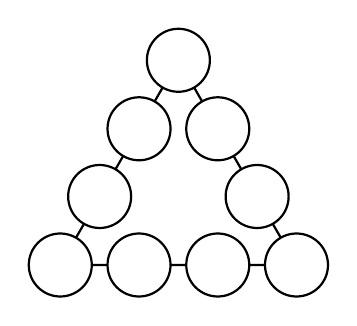
\begin{tikzpicture}
\draw[thick] (0,0) -- (3,0) -- (1.5,2.6) -- cycle;
\draw[thick,fill=white] (0,0) circle (0.4);
\draw[thick,fill=white] (1,0) circle (0.4);
\draw[thick,fill=white] (2,0) circle (0.4);
\draw[thick,fill=white] (3,0) circle (0.4);
\draw[thick,fill=white] (0.5,0.87) circle (0.4);
\draw[thick,fill=white] (1,1.73) circle (0.4);
\draw[thick,fill=white] (1.5,2.6) circle (0.4);
\draw[thick,fill=white] (2,1.73) circle (0.4);
\draw[thick,fill=white] (2.5,0.87) circle (0.4);
\end{tikzpicture}
\end{center}

Each of the numbers $1,2,\ldots,9$ is to be written into one of these circles, so that each circle contains exactly one of these numbers and
\begin{enumerate}[(i)]
\item the sums of the four numbers on each side of the triangle are equal;
\item the sums of squares of the four numbers on each side of the triangle are equal.
\end{enumerate}

Find all ways in which this can be done.

\ans The only solutions are
\begin{center}
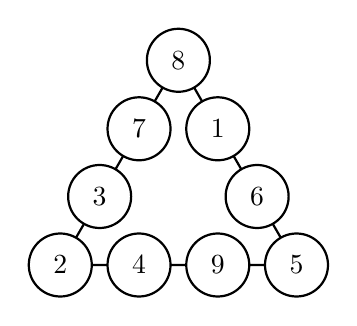
\begin{tikzpicture}
\draw[thick] (0,0) -- (3,0) -- (1.5,2.6) -- cycle;
\draw[thick,fill=white] (0,0) circle (0.4) node {$2$};
\draw[thick,fill=white] (1,0) circle (0.4) node {$4$};
\draw[thick,fill=white] (2,0) circle (0.4) node {$9$};
\draw[thick,fill=white] (3,0) circle (0.4) node {$5$};
\draw[thick,fill=white] (0.5,0.87) circle (0.4) node {$3$};
\draw[thick,fill=white] (1,1.73) circle (0.4) node {$7$};
\draw[thick,fill=white] (1.5,2.6) circle (0.4) node {$8$};
\draw[thick,fill=white] (2,1.73) circle (0.4) node {$1$};
\draw[thick,fill=white] (2.5,0.87) circle (0.4) node {$6$};
\end{tikzpicture}
\end{center}
and the ones generated by permuting the vertices, adjusting sides and exchanging the two middle numbers on each side.

\sol
Let $a$, $b$, and $c$ be the numbers in the vertices of the triangular arrangement. Let $s$ be the sum of the numbers on each side and $t$ be the sum of the squares of the numbers on each side. Summing the numbers (or their squares) on the three sides repeats each once the numbers on the vertices (or their squares):
\begin{gather*}
3s = a+b+c + (1+2+\cdots+9) = a+b+c+45\\
3t = a^2+b^2+c^2 + (1^2+2^2+\cdots+9^2) = a^2+b^2+c^2+285
\end{gather*}

At any rate, $a+b+c$ and $a^2+b^2+c^2$ are both multiples of $3$. Since $x^2\equiv 0,1\pmod 3$, either $a,b,c$ are all multiples of $3$ or none is a multiple of $3$. If two of them are $1,2\bmod 3$ then $a+b+c\equiv 0\pmod 3$ implies that the other should be a multiple of $3$, which is not possible. Thus $a,b,c$ are all congruent modulo $3$, that is,
\[\{a,b,c\} = \{3,6,9\},\quad \{1,4,7\},\quad\text{or}\quad \{2,5,8\}.\]

\smallskip
\emph{Case 1: \{a,b,c\} = \{3,6,9\}}. Then $3t = 3^2+6^2+9^2 + 285 \iff t = 137$.
\begin{center}
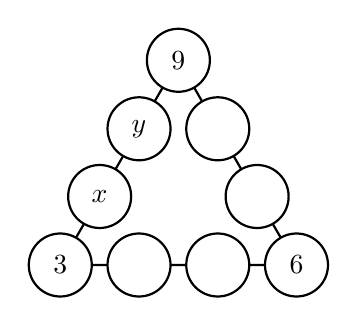
\begin{tikzpicture}
\draw[thick] (0,0) -- (3,0) -- (1.5,2.6) -- cycle;
\draw[thick,fill=white] (0,0) circle (0.4) node {$3$};
\draw[thick,fill=white] (1,0) circle (0.4);
\draw[thick,fill=white] (2,0) circle (0.4);
\draw[thick,fill=white] (3,0) circle (0.4) node {$6$};
\draw[thick,fill=white] (0.5,0.87) circle (0.4) node {$x$};
\draw[thick,fill=white] (1,1.73) circle (0.4) node {$y$};
\draw[thick,fill=white] (1.5,2.6) circle (0.4) node {$9$};
\draw[thick,fill=white] (2,1.73) circle (0.4);
\draw[thick,fill=white] (2.5,0.87) circle (0.4);
\end{tikzpicture}
\end{center}

In this case $x^2+y^2+3^2+9^2 = 137\iff x^2+y^2 = 47$. However, $47$ cannot be written as the sum of two squares. One can check manually, or realize that $47\equiv 3\pmod 4$, and since $x^2,y^2\equiv 0,1\pmod 4$, $x^2+y^2\equiv 0,1,2\pmod 4$ cannot be $47$.

Hence there are no solutions in this case.

\goodbreak
\smallskip
\emph{Case 2: \{a,b,c\} = \{1,4,7\}.} Then $3t = 1^2+4^2+7^2 + 285 \iff t = 117$.
\begin{center}
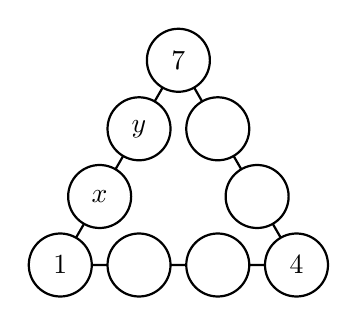
\begin{tikzpicture}
\draw[thick] (0,0) -- (3,0) -- (1.5,2.6) -- cycle;
\draw[thick,fill=white] (0,0) circle (0.4) node {$1$};
\draw[thick,fill=white] (1,0) circle (0.4);
\draw[thick,fill=white] (2,0) circle (0.4);
\draw[thick,fill=white] (3,0) circle (0.4) node {$4$};
\draw[thick,fill=white] (0.5,0.87) circle (0.4) node {$x$};
\draw[thick,fill=white] (1,1.73) circle (0.4) node {$y$};
\draw[thick,fill=white] (1.5,2.6) circle (0.4) node {$7$};
\draw[thick,fill=white] (2,1.73) circle (0.4);
\draw[thick,fill=white] (2.5,0.87) circle (0.4);
\end{tikzpicture}
\end{center}

In this case $x^2+y^2+1^2+7^2 = 117\iff x^2+y^2 = 67\equiv 3\pmod 4$, and as in the previous case there are no solutions.

\smallskip
\emph{Case 3: $\{a,b,c\} = \{2,5,8\}$.} Then $3t = 2^2+5^2+8^2 + 285 \iff t = 126$.
\begin{center}
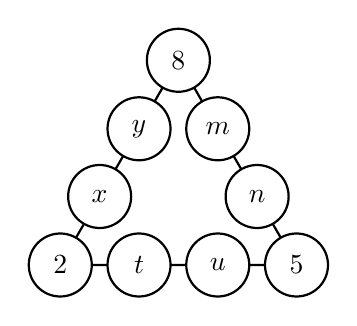
\begin{tikzpicture}
\draw[thick] (0,0) -- (3,0) -- (1.5,2.6) -- cycle;
\draw[thick,fill=white] (0,0) circle (0.4) node {$2$};
\draw[thick,fill=white] (1,0) circle (0.4) node {$t$};
\draw[thick,fill=white] (2,0) circle (0.4) node {$u$};
\draw[thick,fill=white] (3,0) circle (0.4) node {$5$};
\draw[thick,fill=white] (0.5,0.87) circle (0.4) node {$x$};
\draw[thick,fill=white] (1,1.73) circle (0.4) node {$y$};
\draw[thick,fill=white] (1.5,2.6) circle (0.4) node {$8$};
\draw[thick,fill=white] (2,1.73) circle (0.4) node {$m$};
\draw[thick,fill=white] (2.5,0.87) circle (0.4) node {$n$};
\end{tikzpicture}
\end{center}

Then
\[\left\{\begin{matrix}
x^2+y^2+2^2+8^2 = 126\\
t^2+u^2+2^2+5^2 = 126\\
m^2+n^2+5^2+8^2 = 126
\end{matrix}\right.\iff
\left\{\begin{matrix}
x^2+y^2 = 58\\
t^2+u^2 = 97\\
m^2+n^2 = 37
\end{matrix}\right.\]

The only solutions to $t^2+u^2=97$ and $m^2+n^2=37$ are $\{t,u\} = \{4,9\}$ and $\{m,n\} = \{1,6\}$, respectively (again, one can check manually.) Then $\{x,y\} = \{3,7\}$, and the solutions are
\begin{center}
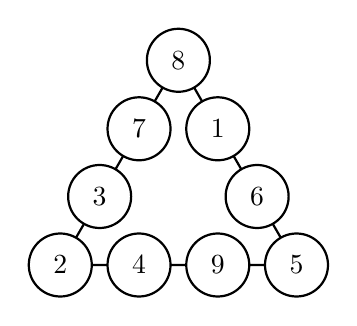
\begin{tikzpicture}
\draw[thick] (0,0) -- (3,0) -- (1.5,2.6) -- cycle;
\draw[thick,fill=white] (0,0) circle (0.4) node {$2$};
\draw[thick,fill=white] (1,0) circle (0.4) node {$4$};
\draw[thick,fill=white] (2,0) circle (0.4) node {$9$};
\draw[thick,fill=white] (3,0) circle (0.4) node {$5$};
\draw[thick,fill=white] (0.5,0.87) circle (0.4) node {$3$};
\draw[thick,fill=white] (1,1.73) circle (0.4) node {$7$};
\draw[thick,fill=white] (1.5,2.6) circle (0.4) node {$8$};
\draw[thick,fill=white] (2,1.73) circle (0.4) node {$1$};
\draw[thick,fill=white] (2.5,0.87) circle (0.4) node {$6$};
\end{tikzpicture}
\end{center}
and the ones generated by permuting the vertices, adjusting sides and exchanging the two middle numbers on each side. There are $3!\cdot 2^3 = 48$ such solutions.

% Problem 3
\prob Let $ABC$ be a triangle. Let $M$ and $N$ be the points in which the median and angle bisector, respectively, at $A$ meet the side $BC$. Let $Q$ and $P$ be the points in which the perpendicular at $N$ to $NA$ meets $MA$ and $BA$, respectively, and $O$ be the point in which the perpendicular at $P$ to $BA$ meets $AN$ produced. Prove that $QO$ is perpendicular to $BC$.

\soln
Let $AN$ meet the circumcircle of $ABC$ at point $K$, the midpoint of arc $BC$ that does not contain $A$.
\begin{center}
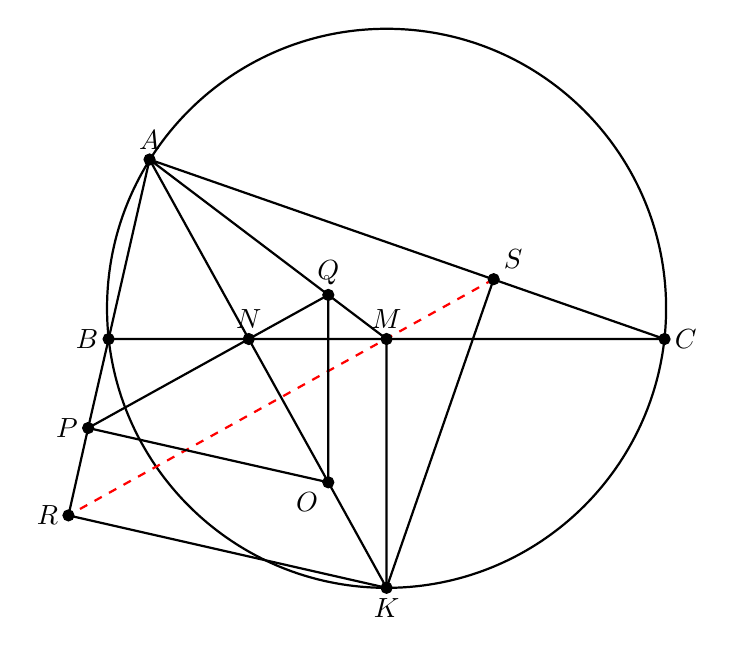
\begin{tikzpicture}
\draw[thick] (0.84,-0.34) node[anchor=south] {$A$} -- (0.32,-2.62) node[anchor=east] {$B$}
    -- (7.38,-2.62) node[anchor=west] {$C$} -- (0.84,-0.34) -- (2.1,-2.62) node[anchor=south] {$N$}
		-- (3.11,-4.44) node[anchor=north east] {$O$} -- (3.85,-5.78) node[anchor=north] {$K$}
		-- (3.85,-2.62) node[anchor=south] {$M$} -- (3.11,-2.06) node[anchor=south] {$Q$} -- (0.84,-0.34);
\draw[thick] (3.85,-2.23) circle (3.55);
\draw[thick] (0.32,-2.62) -- (0.06,-3.75) node[anchor=east] {$P$} -- (3.11,-2.06);
\draw[thick, dashed, color=red] (5.21,-1.86) node[anchor=south west,color=black] {$S$} -- (-0.19,-4.86) node[anchor=east,color=black] {$R$};
\draw[thick] (-0.19,-4.86) -- (0.06,-3.75) -- (3.11,-4.44) -- (3.11,-2.06);
\draw[thick] (-0.19,-4.86) -- (3.85,-5.78) -- (5.21,-1.86);
\draw[fill=black] (5.21,-1.86) circle (2pt);
\draw[fill=black] (-0.19,-4.86) circle (2pt);
\draw[fill=black] (0.84,-0.34) circle (2pt);
\draw[fill=black] (0.06,-3.75) circle (2pt);
\draw[fill=black] (0.32,-2.62) circle (2pt);
\draw[fill=black] (7.38,-2.62) circle (2pt);
\draw[fill=black] (2.1,-2.62) circle (2pt);
\draw[fill=black] (3.11,-4.44) circle (2pt);
\draw[fill=black] (3.85,-5.78) circle (2pt);
\draw[fill=black] (3.85,-2.62) circle (2pt);
\draw[fill=black] (3.11,-2.06) circle (2pt);
\end{tikzpicture}
\end{center}

The orthogonal projection of $K$ onto side $BC$ is $M$. Let $R$ and $S$ be the orthogonal projections of $K$ onto lines $AB$ and $AC$, respectively. Points $R$, $M$, and $S$ lie in the \emph{Simson line} of $K$ with respect to $ABC$. Since $K$ is in the bisector of $\angle BAC$, $ARKS$ is a kite, and the Simson line $RMS$ is perpendicular to $AN$, and therefore parallel to $PQ$.

Now consider the homothety with center $A$ that takes $O$ to $K$. Since $OP\perp AB$ and $KR\perp AB$, $OP$ and $KR$ are parallel, which means that $P$ is taken to $R$. Finally, line $PQ$ is parallel to line $RS$, so line $PQ$ is taken to line $RS$ by the homothety. Then $Q$ is taken to $M$, and since $O$ is taken to $K$, line $OQ$ is taken to line $MK$. We are done now: this means that $OQ$ is parallel to $MK$, which is perpendicular to $BC$ (it is its perpendicular bisector, as $MB=MC$ and $KB=KC$.)

\soln
Consider a cartesian plane with $A=(0,0)$ as the origin and the bisector $AN$ as $x$-axis. Thus $AB$ has equation $y=mx$ and $AC$ has equation $y=-mx$. Let $B = (b,mb)$ and $C = (c,-mc)$. By symmetry, the problem is immediate if $AB=AC$, that is, if $b=c$. Suppose that $b\ne c$ from now on. Line $BC$ has slope $\frac{mb-(-mc)}{b-c} = \frac{m(b+c)}{b-c}$. Let $N = (n,0)$.

Point $M$ is the midpoint $\left(\frac{b+c}2,\frac{mb-mc}2\right)$ of $BC$, so $AM$ has slope $\frac{m(b-c)}{b+c}$.

The line through $N$ that is perpendicular to the $x$-axis $AN$ is $x=n$. Therefore
\[P = (n,mn)\quad\text{and}\quad Q = \left(n,\frac{m(b-c)n}{b+c}\right).\]

In the right triangle $APO$, with altitude $AN$, $AN\cdot AO = AP^2$. Thus
\[n\cdot AO = (0-n)^2 + (0-mn)^2 \iff AO = n(m^2+1)\implies O = (n(m^2+1),0).\]

Finally, the slope of $OQ$ is
\[\frac{\frac{m(b-c)n}{b+c} - 0}{n - n(m^2+1)} = -\frac{b-c}{(b+c)m}.\]

Since the product of the slopes of $OQ$ and $BC$ is
\[-\frac{b-c}{(b+c)m}\cdot\frac{m(b+c)}{b-c}=-1,\]
$OQ$ and $BC$ are perpendicular, and we are done.

\comment
The second solution shows that $N$ can be any point in the bisector of $\angle A$. In fact, if we move $N$ in the bisector and construct $O$, $P$ and $Q$ accordingly, then all lines $OQ$ obtained are parallel: just consider a homothety with center $A$ and variable ratios.

% Problem 4
\prob Let $n,k$ be given positive integers with $n>k$. Prove that
\[\frac1{n+1}\cdot \frac{n^n}{k^k(n-k)^{n-k}} < \frac{n!}{k!\,(n-k)!} < \frac{n^n}{k^k(n-k)^{n-k}}.\]

\sol
The inequality is equivalent to
\[\frac{n^n}{n+1} < \binom nk k^k(n-k)^{n-k} < n^n,\]
which suggests investigating the binomial expansion of
\[n^n = ((n-k)+k)^n = \sum_{i=0}^n \binom ni (n-k)^{n-i}k^i.\]

The $(k+1)$th term $T_{k+1}$ of the expansion is $\binom nk k^k(n-k)^{n-k}$, and all terms in the expansion are positive, which implies the right inequality.

Now, for $1\le i\le n$,
\[\frac{T_{i+1}}{T_i} = \frac{\binom ni (n-k)^{n-i}k^i}{\binom n{i-1} (n-k)^{n-i+1}k^{i-1}}
= \frac{(n-i+1)k}{i(n-k)},\]
and
\[\frac{T_{i+1}}{T_i} > 1 \iff (n-i+1)k > i(n-k)\iff i < k + \frac kn\iff i\le k.\]

This means that
\[T_1 < T_2 < \cdots < T_{k+1} > T_{k+2} > \cdots > T_{n+1},\]
that is, $T_{k+1} = \binom nk k^k(n-k)^{n-k}$ is the largest term in the expansion. The maximum term is greater that the average, which is the sum $n^n$ divided by the quantity $n+1$, therefore
\[\binom nk k^k(n-k)^{n-k} > \frac{n^n}{n+1},\]
as required.

\comment If we divide further by $n^n$ one finds
\[\frac1{n+1} < \binom nk \left(\frac kn\right)^k\left(1-\frac kn\right)^{n-k} < 1.\]

The middle term is the probability $P(X=k)$ of $k$ successes in a binomial distribution with $n$ trials and success probability $p=\frac kn$. The right inequality is immediate from the fact that $P(X=k)$ is not the only possible event in this distribution, and the left inequality comes from the fact that the mode of the binomial distribution are given by $\lfloor (n+1)p\rfloor = \lfloor (n+1)\frac kn \rfloor = k$ and $\lceil (n+1)p-1\rceil = k$. However, the proof of this fact is identical to the above solution.


% Problem 5
\prob Given a permutation $(a_0,a_1,\ldots,a_n)$ of the sequence $0,1,\ldots,n$. A transposition of $a_i$ with $a_j$ is called \emph{legal} if $a_i=0$ for $i>0$, and $a_{i-1} + 1 = a_j$. The permutation $(a_0,a_1,\ldots,a_n)$ is called \emph{regular} if after a number of legal transpositions it becomes $(1,2,\ldots,n,0)$. For which numbers $n$ is the permutation $(1,n,n-1,\ldots,3,2,0)$ regular?

\ans $n=2$ and $n=2^k-1$, $k$ positive integer.

\sol
A legal transposition consists of looking at the number immediately before $0$ and exchanging $0$ and its successor; therefore, we can perform at most one legal transposition to any permutation, and a legal transposition is not possible only and if only $0$ is preceded by $n$.

If $n=1$ or $n=2$ there is nothing to do, so $n=1 = 2^1-1$ and $n=2$ are solutions. Suppose that $n>3$ in the following.

Call a \emph{pass} a maximal sequence of legal transpositions that move $0$ to the left. We first illustrate what happens in the case $n=15$, which is large enough to visualize what is going on. The first pass is
\begin{gather*}
(1,15,14,13,12,11,10,9,8,7,6,5,4,\mathbf{3},2,0)\\
(1,15,14,13,12,11,10,9,8,7,6,\mathbf{5},4,0,2,3)\\
(1,15,14,13,12,11,10,9,8,\mathbf{7},6,0,4,5,2,3)\\
(1,15,14,13,12,11,10,\mathbf{9},8,0,6,7,4,5,2,3)\\
(1,15,14,13,12,\mathbf{11},10,0,8,9,6,7,4,5,2,3)\\
(1,15,14,\mathbf{13},12,0,10,11,8,9,6,7,4,5,2,3)\\
(1,\mathbf{15},14,0,12,13,10,11,8,9,6,7,4,5,2,3)\\
(1,0,14,15,12,13,10,11,8,9,6,7,4,5,2,3)
\end{gather*}

After exchanging $0$ and $2$, the second pass is
\begin{gather*}
(1,2,14,15,12,13,10,11,8,9,\mathbf{6},7,4,5,0,3)\\
(1,2,14,15,12,13,\mathbf{10},11,8,9,0,7,4,5,6,3)\\
(1,2,\mathbf{14},15,12,13,0,11,8,9,10,7,4,5,6,3)\\
(1,2,0,15,12,13,14,11,8,9,10,7,4,5,6,3)
\end{gather*}

After exchanging $0$ and $3$, the third pass is
\begin{gather*}
(1,2,3,15,12,13,14,11,8,9,10,\mathbf{7},4,5,6,0)\\
(1,2,3,15,12,13,14,\mathbf{11},8,9,10,0,4,5,6,7)\\
(1,2,3,\mathbf{15},12,13,14,0,8,9,10,11,4,5,6,7)\\
(1,2,3,0,12,13,14,15,8,9,10,11,4,5,6,7)
\end{gather*}

After exchanging $0$ and $4$, the fourth pass is
\begin{gather*}
(1,2,3,4,\textbf{12},13,14,15,8,9,10,11,0,5,6,7)\\
(1,2,3,4,0,13,14,15,8,9,10,11,12,5,6,7)
\end{gather*}

And then one can successively perform the operations to eventually find
\[(1,2,3,4,5,6,7,0,8,9,10,11,12,13,14,15)\]
after which $0$ will move one unit to the right with each transposition, and $n=15$ is a solution.

The general case follows.

\emph{Case 1: $n>2$ even:} After the first pass, in which $0$ is transposed successively with $3,5,\ldots,n-1$, after which $0$ is right after $n$, and no other legal transposition can be performed. So $n$ is not a solution in this case.

\smallskip
\emph{Case 2: $n=2^k-1$:} Denote $N=n+1$, $R=2^r$, $[a:b] = (a,a+1,a+2,\ldots,b)$, and concatenation by a comma. Let $P_r$ be the permutation
%\begin{gather*}
\[[1:R-1],(0),[N-R:N-1],[N-2R:N-R-1],\ldots,[2R:3R-1],[R:2R-1]\]
%\end{gather*}

$P_r$ is formed by the blocks $[1:R-1],(0)$, and other $2^{k-r}-1$ blocks of size $R=2^r$ with consecutive numbers, beginning with $tR$ and finishing with $(t+1)R-1$, in decreasing order of $t$. Also define $P_0$ as the initial permutation.

Then it can be verified that $P_{r+1}$ is obtained from $P_r$ after a number of legal transpositions: it can be easily verified that $P_0$ leads to $P_1$, as $0$ is transposed successively with $3,5,\ldots,n-1$, shifting cyclically all numbers with even indices; this is $P_1$.

Starting from $P_r$, $r>0$, $0$ is successively transposed with $R, 3R, \ldots, N-R$. The numbers $0, N-R, N-3R, \ldots, 3R, R$ are cyclically shifted. This means that $R$ precedes $0$, and the blocks become
\[\displaylines{
[1:R],(0),[N-R+1:N-1],[N-2R:N-R],[N-3R+1:N-2R-1],\ldots,\cr
[3R+1:4R-1],[2R:3R],[R+1:2R-1]}\]

Note that the first block and the ones on even positions greater than $2$ have one more number and the other blocks have one less number.

Now $0, N-R+1, N-3R+1, \ldots, 3R+1, R+1$ are shifted. Note that, for every $i$th block, $i$ odd greater than $1$, the first number is cyclically shifted, and the blocks become
\[\displaylines{[1:R+1],(0),[N-R+2:N-1],[N-2R:N-R+1],[N-3R+2:N-2R-1],\ldots,\cr
[3R+1:4R-1],[2R:3R+1],[R+2:2R-1]}\]

The same phenomenom happened: the first block and the ones on even positions greater than $2$ have one more number and the other blocks have one less number. This pattern continues: $0, N-R+u, N-3R+u,\ldots, R+u$ are shifted, $u=0,1,2,\ldots,R-1$, the first block and the ones on even positions greater than $2$ have one more number and the other blocks have one less number, until they vanish. We finish with
\[[1:2R-1],(0),[N-2R:N-1],\ldots,[2R:4R-1],\]
which is precisely $P_{r+1}$.

Since $P_k=[1:N-1],(0)$, $n=2^k-1$ is a solution.

\emph{Case 3: $n$ is odd, but is not of the form $2^k-1$.} Write $n+1$ as $n+1 = 2^a(2b+1)$, $b\ge1$, and define $P_0,\ldots,P_a$ as in the previous case. Since $2^a$ divides $N=n+1$, the same rules apply, and we obtain $P_a$:
\[[1:2^a-1],(0),[N-2^a:N-1],[N-2^{a+1}:N-2^a-1],\ldots,[2^{a+1}:3\cdot 2^a-1],[2^a:2^{a+1}-1].\]

But then $0$ is transposed with $2^a, 3\cdot 2^a, \ldots, (2b-1)\cdot 2^a = N-2^{a+1}$, after which $0$ is put immediately after $N-1=n$, and cannot be transposed again. Therefore, $n$ is not a solution.

All cases were studied, and so we are done.

\comment
The general problem of finding the number of regular permutations for any $n$ seems to be difficult. A computer finds the first few values
\[1,2,5,14,47,189,891,4815,29547,\]
which is not catalogued at \href{https://oeis.org/search?q=1%2C2%2C5%2C14%2C47%2C189%2C891%2C4815%2C29547}{oeis.org}.

\end{document}